\section{More Waves}

\underline{\textbf{Part 1}} \par

Choose reasonable values for velocity $v$, amplitude $A$, and wavelength $\lambda$ and reproduce the transverse traveling wave shown in lecture by using springs and masses in Interactive Physics.
Include several snapshots at different points in time.

\vspace{\baselineskip}

Tips: turn gravity off (optional); don't confuse the wave number $k$ with the spring constant $k_s$; consider the initial positions and velocities of each block.

\begin{figure}[H]
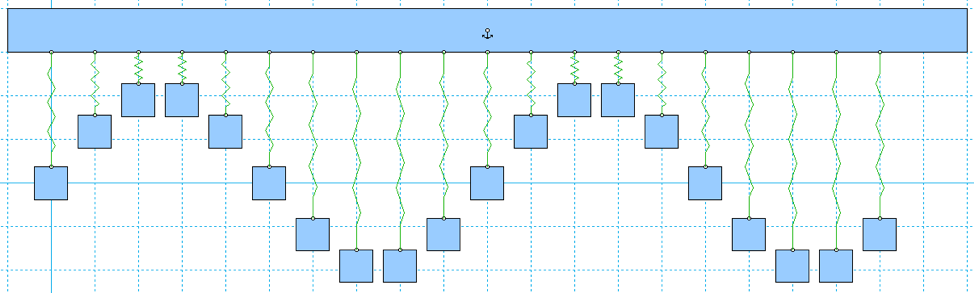
\includegraphics[scale=0.80]{figures/more-waves/fig1.png}
\end{figure}

Write down the function $f(x, t)$ that describes this wave and plot it in SageMath (see previous waves lab for examples).
Save the animated gif as part of your lab report.

\vspace{\baselineskip}

\underline{\textbf{Part 2}} \par

Create a standing wave in SageMath by summing together two traveling waves.
Save the animated gif as part of your lab report.


\pagebreak \clearpage
